%%%%%%%%%%%%%%%%%%%%%%%%%%%%% Define Article %%%%%%%%%%%%%%%%%%%%%%%%%%%%%%%%%%
\documentclass{article}
%%%%%%%%%%%%%%%%%%%%%%%%%%%%%%%%%%%%%%%%%%%%%%%%%%%%%%%%%%%%%%%%%%%%%%%%%%%%%%%

%%%%%%%%%%%%%%%%%%%%%%%%%%%%% Using Packages %%%%%%%%%%%%%%%%%%%%%%%%%%%%%%%%%%
\usepackage{geometry}
\usepackage{graphicx}
\usepackage{amssymb}
\usepackage{amsmath}
\usepackage{amsthm}
\usepackage{empheq}
\usepackage{mdframed}
\usepackage{booktabs}
\usepackage{lipsum}
\usepackage{graphicx}
\usepackage{color}
\usepackage{psfrag}
\usepackage{pgfplots}
\usepackage{bm}
%%%%%%%%%%%%%%%%%%%%%%%%%%%%%%%%%%%%%%%%%%%%%%%%%%%%%%%%%%%%%%%%%%%%%%%%%%%%%%%

% Other Settings

%%%%%%%%%%%%%%%%%%%%%%%%%% Page Setting %%%%%%%%%%%%%%%%%%%%%%%%%%%%%%%%%%%%%%%
\geometry{a4paper}

%%%%%%%%%%%%%%%%%%%%%%%%%% Define some useful colors %%%%%%%%%%%%%%%%%%%%%%%%%%
\definecolor{ocre}{RGB}{243,102,25}
\definecolor{mygray}{RGB}{243,243,244}
\definecolor{deepGreen}{RGB}{26,111,0}
\definecolor{shallowGreen}{RGB}{235,255,255}
\definecolor{deepBlue}{RGB}{61,124,222}
\definecolor{shallowBlue}{RGB}{235,249,255}
%%%%%%%%%%%%%%%%%%%%%%%%%%%%%%%%%%%%%%%%%%%%%%%%%%%%%%%%%%%%%%%%%%%%%%%%%%%%%%%

%%%%%%%%%%%%%%%%%%%%%%%%%% Define an orangebox command %%%%%%%%%%%%%%%%%%%%%%%%
\newcommand\orangebox[1]{\fcolorbox{ocre}{mygray}{\hspace{1em}#1\hspace{1em}}}
%%%%%%%%%%%%%%%%%%%%%%%%%%%%%%%%%%%%%%%%%%%%%%%%%%%%%%%%%%%%%%%%%%%%%%%%%%%%%%%

%%%%%%%%%%%%%%%%%%%%%%%%%%%% English Environments %%%%%%%%%%%%%%%%%%%%%%%%%%%%%
\newtheoremstyle{mytheoremstyle}{3pt}{3pt}{\normalfont}{0cm}{\rmfamily\bfseries}{}{1em}{{\color{black}\thmname{#1}~\thmnumber{#2}}\thmnote{\,--\,#3}}
\newtheoremstyle{myproblemstyle}{3pt}{3pt}{\normalfont}{0cm}{\rmfamily\bfseries}{}{1em}{{\color{black}\thmname{#1}~\thmnumber{#2}}\thmnote{\,--\,#3}}
\theoremstyle{mytheoremstyle}
\newmdtheoremenv[linewidth=1pt,backgroundcolor=shallowGreen,linecolor=deepGreen,leftmargin=0pt,innerleftmargin=20pt,innerrightmargin=20pt,]{theorem}{Theorem}[section]
\theoremstyle{mytheoremstyle}
\newmdtheoremenv[linewidth=1pt,backgroundcolor=shallowBlue,linecolor=deepBlue,leftmargin=0pt,innerleftmargin=20pt,innerrightmargin=20pt,]{definition}{Definition}[section]
\theoremstyle{myproblemstyle}
\newmdtheoremenv[linecolor=black,leftmargin=0pt,innerleftmargin=10pt,innerrightmargin=10pt,]{problem}{Problem}[section]
%%%%%%%%%%%%%%%%%%%%%%%%%%%%%%%%%%%%%%%%%%%%%%%%%%%%%%%%%%%%%%%%%%%%%%%%%%%%%%%

%%%%%%%%%%%%%%%%%%%%%%%%%%%%%%% Plotting Settings %%%%%%%%%%%%%%%%%%%%%%%%%%%%%
\usepgfplotslibrary{colorbrewer}
\pgfplotsset{width=8cm,compat=1.9}
%%%%%%%%%%%%%%%%%%%%%%%%%%%%%%%%%%%%%%%%%%%%%%%%%%%%%%%%%%%%%%%%%%%%%%%%%%%%%%%

%%%%%%%%%%%%%%%%%%%%%%%%%%%%%%% Title & Author %%%%%%%%%%%%%%%%%%%%%%%%%%%%%%%%
\title{SoccerSim}
\author{Gabriel Yuseff}
%%%%%%%%%%%%%%%%%%%%%%%%%%%%%%%%%%%%%%%%%%%%%%%%%%%%%%%%%%%%%%%%%%%%%%%%%%%%%%%

\begin{document}
    \maketitle
    \section{Introduction}
    \vspace{1px}
    I want to practice my coding skills. So I will create a Soccer simulator, based one of my first homeworks in Advanced Programming; which was a console Quiddich match simulator.\\
    For the project I want to try and use several of the things I learned afterwards in the course.\\
    I'll do it in C\# as I used that language in the course, however I could also try doing it in Python or C++.\\
    PS: This will also help me remember how to write TEX files
    \newpage
    \section{Project Definitions}
    
    \subsection{What I want to do}

    Here are some ideas that I want to try:
    \begin{itemize}
        \item Simulate a Soccer game with most of its rules
        \item Each player behaves independently following certain logic:
        \begin{itemize}
            \item What is the role of the player (Goalkeeper, Defender, Midfield, Attacker)
            \item The team is attacking or defending
            \item What is the position of the player
            \item What are the positions of the other player 
        \end{itemize}
        \item Make it chance-based for decisions and outcomes
        \begin{itemize}
            \item A player could try to make a difficult shot to the net, instead of an easy (and more intelligent) pass
            \item The player may miss a pass to a teammate that is alone
            \item A Goalkeeper may make score a goal by mere chance
        \end{itemize}
        \item Add stats to the players, which will increase their success chances for the plays
        \item Show all in a simple graphical way
        \item Maybe add user intervention by creating players of its own
        \item Maybe add a tournament mode
    \end{itemize}

    \subsection{What I want to remember}
    For This project I want to use these concepts (at least):
    \begin{itemize}
        \item OOP
        \item Graphical Interfases $\rightarrow$ .NET: Windows Presentation Foundation (WPF)
        \item MultiThreading
        \item Polymorphism
    \end{itemize}
    
    \newpage
    \subsection{What I want to show}
    Use a very basic way to show the game:
    \begin{itemize}
        \item Have a fixed background
        \item The ball and players represented with simple sprites (circles)
        \item Have the score and time showing in a corner
    \end{itemize}

    \begin{figure}[h]
        \begin{center}
            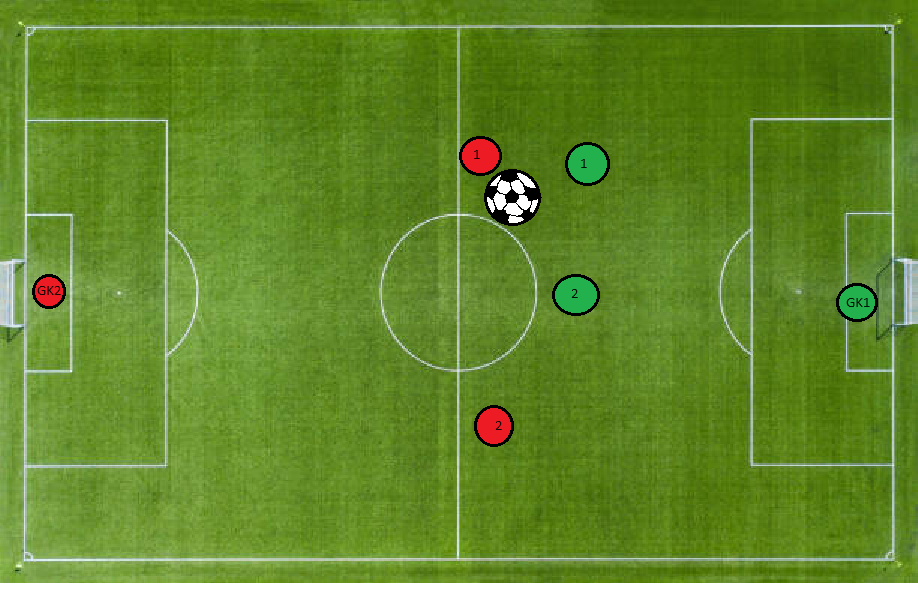
\includegraphics[width=0.7\textwidth]{Images/prototype.png}        
        \end{center}
    \end{figure}
    
    \section{Class definitions}
    \subsection{Players}
    Abstract class: Will be used as a parent class for all the different players. It will contain the base attributes and methods, that will be overwritten by each specific player, class.
    \subsubsection{Attributes}
    \begin{itemize}
        \item ID: Unique ID for each player
        \item Name: Name of the player
        \item Number: The number of the player
        \item Team: Team to which the player belongs
        \item Role: What is the role of this player
        \item Init\_Position: Position the player starts in the match
        \item Pass\_stat: Stat that determines how good they are at passes
        \item Shot\_stat: Stat that determines how good they are at shooting at the net
        \item Tackle\_stat: Stat that determines how good they are at stealing the ball from an opponent
        \item Dribble\_stat: Stat that determines how good they are at keeping the ball when an opponent is trying to take it from theorem
        \item Save\_stat: Stat that determines how good they are at catching a ball thrown to the net
        \item Speed\_stat: Stat that determines how fast can they move
        \item Position: Current position of the player in the field
    \end{itemize}

    \subsubsection{Methods}
    \begin{itemize}
        \item Constructor: Will take all the attributes to create the player
        \item Update: Main method of the Player class. It determines how the player will act in each iteration. It will be dependant on the role, the ball position, the other players positions, who has the ball, etc
        \item Move: Method to translate the player in the field. It depends on the current position and the player velocity
        \item Pass: Method to pass the ball to a teammate
        \item Shot: Method to shot the ball to the opponent team net
        \item Steal: Method to steal the ball from the current owner of the ball. Has a chance to be foul 
    \end{itemize}

    \subsection{Team}
    This are the teams playing the match
    \subsubsection{Attributes}
    \begin{itemize}
        \item ID: Unique id for the team
        \item Name: Name of the Team
        \item Color: Colour of the team
        \item Player: The players in the team
        \item Points: The points that the team has accumulated (if running in a tournament mode)
    \end{itemize}
    \subsubsection{Methods}
    \begin{itemize}
        \item Update: Main method of the team. It starts the threads of the players and updates the status of the team to the match.
        \item Setup: Sets the player in the field on their initial positions
    \end{itemize}

    \subsection{Match}
    The class for the match
    \subsubsection{Attributes}
    \begin{itemize}
        \item Teams: Teams participating in the match
        \item Scores: Scores of each team in the match
        \item Time: Current time of the match
        \item Max time: Total duration of the match
        \item Events: List of events that occured during the match
    \end{itemize}
    
    \subsubsection{Methods}
    \begin{itemize}
        \item Update: Update the state of the match
        \item Print\_GUI: Method to update the GUI
    \end{itemize}

\end{document}